\section{Background}
\label{sec:compiler:background}

\subsection{A Brief Introduction to CompCert}

\myparagraph{Undefined Behavior}
\todo{TODO}

\myparagraph{\cc{} Memory Model}

\myparagraph{Memory Relations of \ccm{}}
\label{sec:overview-verification:injection}

\ccm{} uses the original memory identity and extension of \cc{}
(\Cref{sec:overview-verification:injection:original}) and mildly
strengthens the original memory injection to reason about dynamically allocated
local memory such as a function's stack frame for \emph{open} modules,
which can be compared to the structured injection of \ccc{}
(\Cref{sec:overview-verification:injection:dynamic}).
Moreover, we generalize it further to reason about statically allocated local memory
such as static variables of C by allowing module-local invariants on those static variables
(\Cref{sec:overview-verification:injection:static}).

%% and mildly generalize the memory injection of \cc{} in two steps: first to reason
%% about dynamic local memory such as a function's stack frame
%% (\Cref{sec:overview-verification:injection:dynamic}) and further to
%% reason about static local memory such as static variables of C
%% (\Cref{sec:overview-verification:injection:static}).
%% Structured injections of \ccc{} can be compared to our first generalization

\myparagraph{Memory Relations of \cc{}}
\label{sec:overview-verification:injection:original}
\todo{it was sub-bullet of the above: Memory Relations of \ccm{}}
%
\cc{}'s memory model consists of a finite set of blocks of finite size
and a pointer value (or, an address) is a pair $(b,o)$ of a block id $b$ and an offset $o$ inside it.
The memory identity imposes that the source and target memories are identical;
and the extension that the two memories contain identical block ids and
each target block extends the corresponding source block
with more space and any values in it at the end.

A memory injection injects a subset of the source blocks into target blocks
without overlap. More precisely, a (selected) whole source block is injected into a single target block
while allowing multiple source blocks to be injected into the same target block without overlap.
This injection map specifies the \emph{public} areas of the source and target memories and the correspondence between them.
In other words, the corresponding addresses by the injection map are treated as \emph{equivalent} (public) pointer values,
%% and therefore
so that at those corresponding addresses,
only equivalent%
\footnote{Technically speaking, \cc{} allow more undefined values in the source
  because it proves refinement rather than equivalence between the source and target programs.}
values (\ie equivalent non-pointer values or corresponding addresses) should be stored .
All the areas that are not on the injection map are considered as \emph{private} areas of the source and target memories.





\subsection{Interaction Semantics}

We give a brief overview of interaction semantics of \ccc{}, which
interactively executes modules equipped with their own independent
module semantics. Each module semantics $M$ provides
a set of module states (also called \emph{cores}) $\States{M}$ with the following operations:
\begin{itemize}
\item \texttt{init\_core}: given a function $f$ with arguments $\vec{v}$,
  %and a memory $m$,
  gives the initial module state $s \in \States{M}$
  % with updated memory $m'$
  executing the invoked function $f$ with $\vec{v}$.
\item \texttt{at\_external}: given $s \in \States{M}$,
  %and a memory $m$,
  checks if an external function $f$ is called with arguments~$\vec{v}$.
  %% and if so, gives updated memory $m'$ and state $s'$.
\item \texttt{after\_external}: given $s \in \States{M}$
  where an external function is called,
  %a memory $m$
  and a return value $r$,
  gives the module state $s'$
  %and memory $m'$
  after the function call returns $r$.
\item \texttt{halted}: given $s \in \States{M}$, checks if the module execution is halted with a return value~$r$.
\item \texttt{corestep}: given $s \in \States{M}$ and memory $m$, takes a local step producing an event $e$ and the next state~$s'$ with updated memory $m'$.
\end{itemize}

We explain how interaction semantics works using an example in
\Cref{fig:inter-sem}, where the whole machine state consists of a
memory, say $m$, and a stack of module states (called \emph{core stack}), say $[s_2; s_1]$.
Then, interaction semantics checks whether the stack-top module $s_2$
is invoking an external function using \texttt{at\_external}, and if
so, pushes the invoked module's initial state, say $s_3$, obtained by
\texttt{init\_core}. Note here that the same module $M_1$ can have
multiple module states $s_1$ and $s_3$ in the stack.  Then the
new top module $s_3$ takes a local step to $s_3'$ with updated memory
$m'$ according to its \texttt{corestep}, and if $s_3'$ is a halted
state with a return value $r$ (checked with \texttt{halted}), the top
module $s_3'$ is popped and returned to the next module $s_2$, which
is then updated to $s_2'$ given by \texttt{after\_external} with the return
value $r$.

\begin{figure}[t]
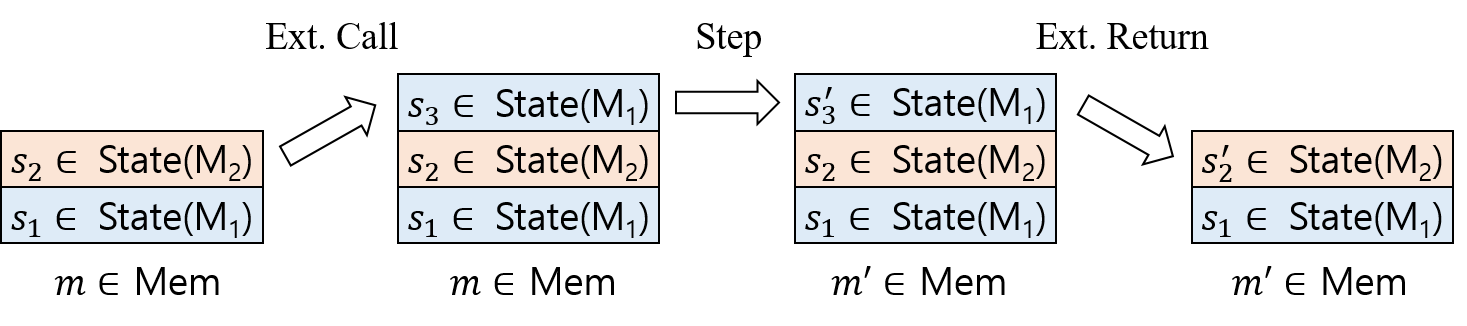
\includegraphics[width=0.9\linewidth]{images/intersem.png}
\caption{An execution of interaction semantics}
\label{fig:inter-sem}
\end{figure}

%% marshalling unmarshalling
%% marshalling the argument values into a list of values
%% setting the initial core states, unmarshalling the list of arguments.
%% at\_external: marshalling the argument values into a list of values
%% after\_external: unmarshalling the return value into
%% halted: marshalling the return value
%% corestep: use the underlying language semantics

Finally, note that the language semantics of C, assembly and
intermediate languages can be lifted to give a module semantics by
defining \texttt{corestep} to be the same as the execution step of the
language's semantics, and the other module operations to reflect the
calling conventions. Note also that all language-specific resources
(\ie other than the memory)
such as the register-file of assembly 
reside inside the module state, and thus are
duplicated at each invocation of a module.

%% One can lift a \cc{} language semantics into a core semantics by providing the interfaces:
%% Note that it is possible to define a core semantics using a mathematical specification.
